\documentclass[../main.tex]{subfiles}
\begin{document}


\section{How to write thesis
chapters}\label{how-to-write-thesis-chapters}

Quarto uses markdown syntax. I use Rstudio as my IDE. \textbf{knitr} is
the engine that interprets code chunks when using Rstudio, and it
supports a variety of languages, including R, Python, SQL, JavaScript,
and Ruby. For a full list of supported languages, type the following
command:

\texttt{names(knitr::knit\_engines\$get())}

Citations are done like this \cite{strain_2023}, and point to
references.bib in the parent directory.

\section{Using code chunks}\label{using-code-chunks}

Code chunks can be inserted using a button in the top right corner of
this window, or by using \texttt{Alt+shift+I}. Have a look at
\texttt{example\_chapter.qmd} in \texttt{quarto\_chapters} for a demo of
this. Figure~\ref{fig-example} is produced using an r code chunk.

\begin{figure}

\centering{

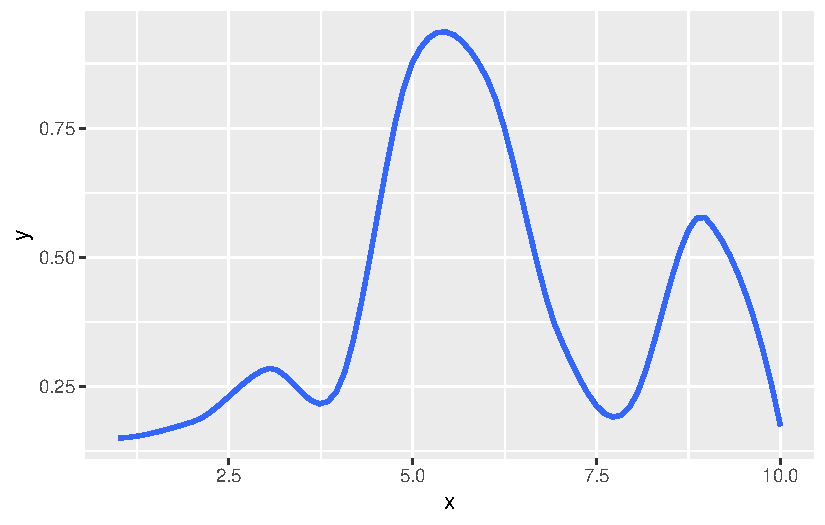
\includegraphics{example_chapter_files/figure-latex/fig-example-1.pdf}

}

\caption{\label{fig-example}An example of a figure}

\end{figure}%

\section{Using other languages}\label{using-other-languages}

To use other languages, simply label the chunk accordingly. Doing this
will require installation of the appropriate package - using python
requires the \texttt{reticulate} package.

For an example, see the .qmd file associated with this chapter.

You can mix and match different languages throughout your report.

\section{Models}\label{models}

Knitr includes the ability to cache models. This is very useful if your
models are especially complex or you have a very large report. This is
demonstrated below.

Setting eval\_models to TRUE in line 9 means models are evaluated and
cached with every knit. Setting to false means that knitr looks for the
model in the cache, so you only have to set it once! The chunk below
accomplishes this:

\section{Using this template}\label{using-this-template}

\begin{itemize}
\tightlist
\item
  chapters should be written using quarto markdown and are located in
  the \texttt{chapters\_quarto} folder.
\item
  \texttt{main.tex} in the top-level directory should be used to specify
  authors, declarations, abstracts etc.
\item
  once chapters are all written, reformat the tex using the function
  provided in the \texttt{reformat\_tex.r} file, then compile
  \texttt{main.tex}.
\end{itemize}

Itemise is demonstrated above.

\section{Labelling}\label{labelling}

Chapters are referenced as such:

\chap{chap:example_chapter}

As in, in \chap{chap:example_chapter}\ldots{}

Sections are labelled similarly, but you need to type the word
``Section'' in addition.

As in, in Section \ref{labelling}\ldots{}

You will probably end up with multiple sections called ``Introduction'',
``Methods'', ``Results'' etc. If this is the case, you can manually
specify the label for a section like so:

\section{Introduction\_test}\label{introduction_test}

\section{Introduction\_test}\label{introduction_test2}

In Section \ref{introduction_test} as opposed to Section
\ref{introduction_test2}

\begin{verbatim}
# Introduction_test 

# Introduction_test {#introduction_test2}

In Section \ref{introduction_test} as opposed to Section \ref{introduction_test2}
\end{verbatim}

In Section \ref{introduction_test} as opposed to Section
\ref{introduction_test2}

\section{Labelling Figures}\label{labelling-figures}

\texttt{Figures\ are\ labelled\ as\ so:\ in\ @fig-example,\ we\ can\ see...}

Figures are labelled as so: in Figure~\ref{fig-example}, we can
see\ldots{}

If you are not generating figures from code, but rather including them
using knitr::include\_graphics(), you must set the out-height and
out-width to NA to prevent LaTeX from trying to manually size them.

\section{Lists}\label{lists}

Lists use normal markdown syntax. Unnumbered lists are as so:

here's a list:

\begin{itemize}
\tightlist
\item
  item 1
\item
  items 2
\end{itemize}

And numbered lists:

\begin{enumerate}
\def\labelenumi{\arabic{enumi}.}
\tightlist
\item
  item 1
\item
  item 2
\end{enumerate}




\end{document}
